\documentclass{beamer}

\usepackage{amsmath}
%\usepackage{color}
\usepackage{tikz}
%\usepackage{graphicx}
%\usepackage{concmath}
\usepackage{pifont}
%\usepackage{setspace}
%\usepackage{enumitem}
%\usepackage{verbatim} 
%\usepackage{multirow}
\usetikzlibrary{arrows,positioning,matrix,shapes,chains,calc}

\usepackage{caption}
\captionsetup{labelformat=empty,labelsep=none}

\usetheme{default}
\usefonttheme{serif}
\usefonttheme{professionalfonts}
\beamertemplatenavigationsymbolsempty
\setbeamertemplate{blocks}[rounded][shadow=true]

\definecolor{Red}{rgb}{0.855,0.0,0.039}
\definecolor{orangered}{rgb}{1,0.10,0}
\definecolor{Blue}{rgb}{0.0,0.235,0.561}
\definecolor{DarkBlue}{rgb}{0.0,0.235,0.561}
\definecolor{Grey}{rgb}{0.255,0.259,0.224}
\definecolor{LBlue}{cmyk}{0.1,0.05,0,0}
\definecolor{LGreen}{cmyk}{0.1,0,0.1,0}
\definecolor{LRed}{cmyk}{0,0.1,0,0}
\definecolor{DarkGreen}{rgb}{0,0.4,0}
\definecolor{DarkTurquiose}{rgb}{0.382,0.307,1}
 
\graphicspath{{Images/}}

%--------------------------------------
% Theorem definitions
%--------------------------------------
\theoremstyle{definition}
\newtheorem{thm}[theorem]{Theorem}
\newtheorem{conjecture}[theorem]{Conjecture}
\newtheorem{cor}[theorem]{Corollary}
\newtheorem{prop}[theorem]{Proposition}
\newtheorem{quest}{Question}
\newtheorem{defn}{Definition}
\newtheorem{mthm}{Main Theorem}
  
\newcommand{\putbox}[1]{\begin{equation*}\addtolength{\fboxsep}{5pt}\boxed{\begin{gathered}#1\end{gathered}} \end{equation*}}
\newcommand{\mS}{\mathcal{S}}
\newcommand{\mA}{\mathcal{A}}
\newcommand{\mB}{\mathcal{B}}
\newcommand{\mC}{\mathcal{C}}
\newcommand{\mD}{\mathcal{D}}
\newcommand{\mE}{\mathcal{E}}
\newcommand{\bi}{\mathbf{i}}
\newcommand{\bz}{\mathbf{z}}
\newcommand{\by}{\mathbf{y}}
\newcommand{\oz}{\overline{z}}
\newcommand{\oy}{\overline{y}}
\newcommand{\ox}{\overline{x}}
\newcommand{\bo}{\mathbf{1}}
\newcommand{\ok}{\ensuremath{\overline{k}}}
\newcommand{\sgn}{\text{sgn}}
\newcommand{\mV}{\mathcal{V}}
\newcommand{\bp}{\mbox{\boldmath$\rho$}}


\titlegraphic{
\includegraphics[scale=0.18]{title.jpg}}


\title{Password Authenticated Key Exchange:\\ From Two Party Methods to Group Schemes \vspace{-0.2in}}
\author{Stephen Melczer, Taras Mychaskiw, and Yi Zhang}
\date{}

\begin{document}
\frame{\titlepage}



%%%%%%%%%%%%%%%%%%%%%%%%%%%%%%%%%%%
% Introduction
%%%%%%%%%%%%%%%%%%%%%%%%%%%%%%%%%%%

\frame{  
  \frametitle{Introduction}
  \begin{enumerate}
  \item Classical Two Party PAKEs
  		\begin{enumerate}
  		\item Background and Security Properties
  		\item J-PAKE
  		\item Dragonfly
  		\item PAK/PPK
  		\end{enumerate}
  \item[]
  \item Extension to Group Setting (GPAKEs)
  		\begin{enumerate}
  		\item Fairy-Ring Dance
  		\item Examples of GPAKEs
  		\end{enumerate}
    \item[]
  \item Timings
    \item[]
  \item Conclusion
  \end{enumerate}
}

%%%%%%%%%%%%%%%%%%%%%%%%%%%%%%%%%%%
% Two Party PAKEs
%%%%%%%%%%%%%%%%%%%%%%%%%%%%%%%%%%%

\frame{
  \frametitle{\vspace{1.1in} \begin{center} PART 1 \\ Classical Two Party PAKEs \end{center}}
}


\frame{  
  \frametitle{Password Authenticated Key Exchange (PAKE)}
  PAKEs allow two parties sharing a \emph{short/weak} password to establish a shared key
  \vspace{0.5in}

  Cannot broadcast password directly -- would need to be protected (expensive)
  \vspace{0.5in}

  Instead, modern PAKEs use \emph{zero-knowledge proof} of password in protocol
}

\frame{  
  \frametitle{First Protocol: EKE (Bellovin and Merrit 1992)}
  Pick prim. root $\alpha \in \mathbb{Z}_p$
  \vspace{0.4in}

  \scalebox{0.7}{
    \begin{tikzpicture}
        \matrix (m)[matrix of nodes, column sep=2cm, row sep=8mm, nodes={draw=none, anchor=center, text depth=0pt},ampersand replacement=\&]{
            Alice                                       \&                   \& Bob                                       \\
            randomly choose $x_a \in \mathbb{Z}_p^*$    \& $[\alpha^{x_a}]_s$\&                                           \\
                                                        \& $[\alpha^{x_b}]_s$\& randomly choose $x_b \in \mathbb{Z}_p^*$  \\
        };

        % draw the nodes - these are 1-based indicies on the matrix called `m`, ie to draw in (x,y), reference it as `m-x-y`
        \draw[shorten <=-1.5cm,shorten >=-1.5cm] (m-1-1.south east)--(m-1-1.south west);    % underline "Alice"
        \draw[shorten <=-1.5cm,shorten >=-1.5cm] (m-1-3.south east)--(m-1-3.south west);    % underline "Bob"
        \draw[shorten <=-1cm,shorten >=-1cm,-latex] (m-2-2.south west)--(m-2-2.south east); % arrow below sending alpha^x_a
        \draw[shorten <=-1cm,shorten >=-1cm,-latex] (m-3-2.south east)--(m-3-2.south west); % arrow below sending alpha^x_b
    \end{tikzpicture}}
    \vspace{0.2in}

	Alice and Bob share $K = \alpha^{x_a \cdot x_b}$.    
    \vspace{0.6in}

\pause
Uses password directly $\implies$ many insecurities found
\vspace{0.2in}

\pause
Ex: Decypher $[\alpha^{x_a}]_{s'}$ -- rule out $s'$ if output in $[p,2^{n}-1]$
}

\frame{  
  \frametitle{Desired Security Properties}
  \begin{itemize}
  \item[] \textbf{Offline dictionary attack resistance}
  \item[] Don't leak info which can be used in brute force search
  \item[]
  \item[] \textbf{Forward secrecy for established keys}
  \item[] Past keys secure if password disclosed
  \item[] Implies passive attacker w/ password cannot compute key
  \item[]
  \item[] \textbf{Known session security}
  \item[] All secrets of one session reveals nothing about others
  \item[]
  \item[] \textbf{Online dictionary attack resistance}
  \item[] Attacker can only test one password per protocol execution
  \end{itemize}


}

\frame{  
  \frametitle{J-PAKE}

   \begin{itemize}
 \item[\textbf{Setup}] Let $G = <\hspace{-.05in} g \hspace{-.05in} >$ be an order $q$ subgroup of $\mathbb{Z}_p^*$
 \item[] Alice picks $x_1 \in_R [0,q-1]$ and $x_2 \in_R [1,q-1]$
 \item[] Bob picks $x_3 \in_R [0,q-1]$ and $x_4 \in_R [1,q-1]$
 \item[]\pause
 \item[\textbf{Rd 1}] Alice sends $g^{x_1},g^{x_2}$ and ZKPs of $x_1$ and $x_2$ to Bob
 \item[] Bob sends $g^{x_3},g^{x_4}$ and ZKPs of $x_3$ and $x_4$ to Alice
 \item[] [Alice and Bob verify ZKPs and $g^{x_2},g^{x_4} \neq 1$]
 \item[]\pause
 \item[\textbf{Rd 2}] Alice sends $A = g^{(x_1+x_3+x_4)x_2\cdot s}$ and ZKP of $x_2 s$
 \item[] Bob sends $B = g^{(x_1+x_2+x_3)x_4\cdot s}$ and ZKP of $x_4 s$
 \item[] \pause
 \end{itemize}
  
  They share
  \[ K = \underbrace{\left(B / g^{x_2x_4 s} \right)^{x_2}}_\text{Computable by Alice} = g^{(x_1+x_3)x_2x_4s} = 
 \underbrace{\left(A / g^{x_2x_4 s} \right)^{x_4}}_\text{Computable by Bob}. \]
}

\frame{  
  \frametitle{J-PAKE}
   Satisfies all 4 desired properties \\
   (under DDH and CDH assumptions)
   \vspace{0.4in}

   Only two rounds of communication
   \vspace{0.4in}

   No \emph{explicit} key confirmation (only implicit)
   \vspace{0.4in}

   Not patented
}

\frame{  
  \frametitle{Dragonfly}
  \begin{itemize}
    \item[\textbf{Setup}] Let $Q$ be a cyclic subgroup of $\mathbb{Z}_p^*$ with prime order $q$.
    \item[] Alice picks $r_A, m_A \in_R \mathbb{Z}_q^*$
    \item[] Bob picks $r_B, m_B \in_R \mathbb{Z}_q^*$
    \item<2->[\textbf{Rd 1}] Alice sends $s_A = r_A + m_A \mod q$ and $E_A = \pi^{-m_A} \mod p$
    \item<2->[] Bob sends $s_B = r_B + m_B \mod q$ and $E_B = \pi^{-m_B} \mod p$
    \item<2->[] [Alice and Bob check that $s_A \neq s_B$ or $E_A \neq E_B$]
    \item<3->[\textbf{Rn 2}] Alice computes $ss = (\pi^{s_B} E_B)^{r_A} = \pi^{r_A r_B}$
    \item<3->[] Bob computes $ss = (\pi^{s_A} E_A)^{r_B} = \pi^{r_A r_B}$
    \item<3->[] Alice sends $H(ss | E_A | s_A | E_B | s_B)$
    \item<3->[] Bob sends $H(ss | E_B | s_B | E_A | s_A)$
    \item<3->[] Each member confirms the hashes.
  \end{itemize}
  \uncover<4>{
      They share:
      \[ K = H(ss | E_A \times E_B | (s_A + s_B) \mod q) \]
  }
}

\begin{frame}{Dragonfly}
   No formal security proofs, but claims resistance to offline dictionary attacks
   \vspace{0.4in}

   Only two rounds of communication
   \vspace{0.4in}

   Very fast compared to other protocols
\end{frame}

\frame{  
  \frametitle{PAK/PPK}
  Desciption of protocol
  \vspace{0.3in}

  Security properties
  
}


%%%%%%%%%%%%%%%%%%%%%%%%%%%%%%%%%%%
% GPAKEs
%%%%%%%%%%%%%%%%%%%%%%%%%%%%%%%%%%%

\frame{
  \frametitle{\vspace{1.1in} \begin{center} PART 2 \\ Extension to Group Setting \end{center}}
}

\frame{  
  \frametitle{The Fairy-Ring Dance}
  Desciption of general procedure
  \vspace{0.3in}

  How pairwise + group keys are constructed
}

\frame{  
  \frametitle{J-PAKE+}
  Description of J-PAKE+
  \vspace{0.3in}

  Uses 3 rounds as J-PAKE does not have explicit key confirmation
}

\frame{  
  \frametitle{Dragonfly+}
  Description of Dragonfly+
  
}

\frame{  
  \frametitle{PPK+}
  Description of PPK+
  
}

%%%%%%%%%%%%%%%%%%%%%%%%%%%%%%%%%%%
% Timings
%%%%%%%%%%%%%%%%%%%%%%%%%%%%%%%%%%%

\frame{
  \frametitle{\vspace{1.1in} \begin{center} PART 3 \\ Timings \end{center}}
}

\frame{  
  \frametitle{Specifications}
  \begin{itemize}
    \item All protocol benchmarks were implemented in Java 1.6 and run on a server (3GHz AMD processor, 6GB of RAM) running Ubuntu 12.04.
    \item Benchmarks measured latency, the amount of work each device would have to do in the group excluding communication.
  \end{itemize}
}

\frame{  
  \frametitle{Results}

\begin{centering}
  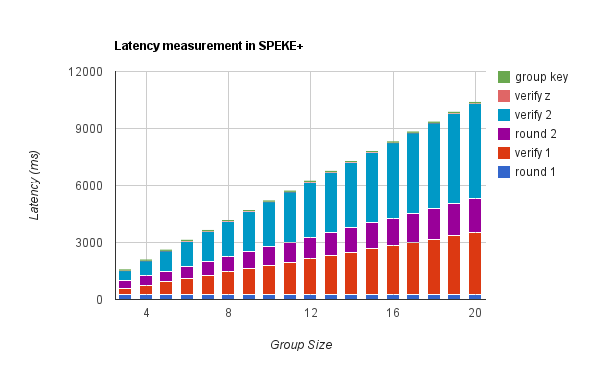
\includegraphics[scale=0.28]{speke.png}
  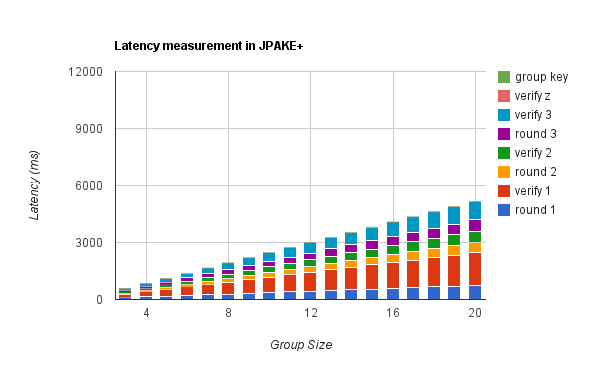
\includegraphics[scale=0.28]{scale_jpake.png}
  \end{centering}

  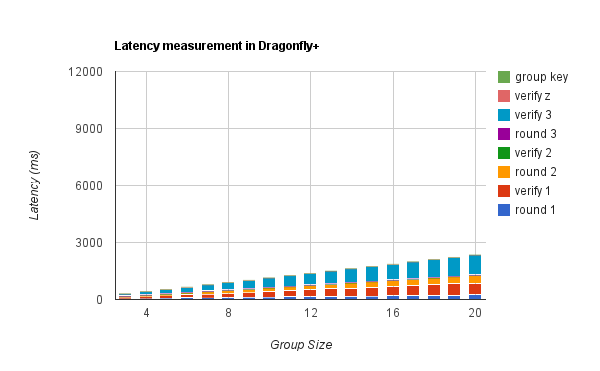
\includegraphics[scale=0.28]{scale_dragon.png}
  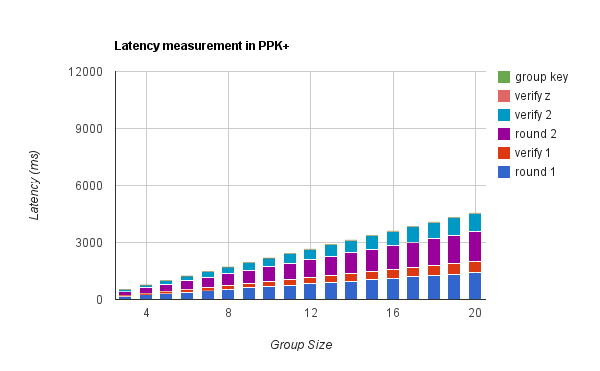
\includegraphics[scale=0.28]{scale_ppk.png}
  
}


%%%%%%%%%%%%%%%%%%%%%%%%%%%%%%%%%%%
% Conclusion
%%%%%%%%%%%%%%%%%%%%%%%%%%%%%%%%%%%

\frame{
  \frametitle{\vspace{1.1in} \begin{center} Conclusion \end{center}}
}

\frame{  
  \frametitle{Conclusion}
  \begin{itemize}
  \item[] It is possible to transfer PAKEs into GPAKEs while preserving round efficiency
  \item[]
  \item[] SPEKE+ is very slow
  \item[]
  \item[] J-PAKE+ is a bit slow, but proven secure (under CDH)
  \item[]
  \item[] PPK is faster but weaker security proof
  \item[]
  \item[] Dragonfly is fastest, but no security proof 
  \item[] (despite IEEE 802.11-2012 standard)
  \end{itemize}
}



\frame{
  \frametitle{\vspace{1.1in} \begin{center} THANK YOU \end{center}}
}

\end{document}


